\section{Validating rain appearance}

We now validate the appearance of our synthetic rainy images when using either of our rain augmentation pipelines.
We observe visual results and quantify their perceptual realism by comparing them to existing rain augmentation approaches.

\subsection{Qualitative evaluation}
\begin{figure}
 \footnotesize
 \setlength{\tabcolsep}{0.025cm}
 \renewcommand{\arraystretch}{0.5}
 \begin{tabular}{ccc}
  \multicolumn{3}{c}{\textbf{Rain photographs}} \\
  & \adjincludegraphics[width=0.44\linewidth,trim={0 {0.50\height} 0 0},clip]{figures/results/qualitative_rain/real/real_rain_putine_crop2.jpg} 
  & \adjincludegraphics[width=0.44\linewidth,trim={0 {0.39\height} 0 0},clip]{figures/results/qualitative_rain/real/real_rain_Luo-xu.jpg}\\
  & \adjincludegraphics[width=0.44\linewidth,trim={{0.1\width} {0.15\height} {0.1\width} {0.15\height}},clip]{figures/results/real_rain/rain/000787.jpg} 
  & \adjincludegraphics[width=0.44\linewidth,trim={{0.1\width} {0.05\height} {0.1\width} {0.30\height}},clip]{figures/results/qualitative_rain/real/rain_dashcam.png}\\
  \toprule
  \multicolumn{3}{c}{\textbf{Our rain rendering}} \\
  \multirow{1}{*}[1.2cm]{\rotatebox{90}{~} \rotatebox{90}{Clear}} & \adjincludegraphics[width=0.45\linewidth,trim={{0.1\width} {0.1\height} {0.1\width} {0.1\height}},clip]{figures/results/qualitative_rain/nuscenes/clear/001.jpg} & \adjincludegraphics[width=0.45\linewidth,trim={{0.1\width} {0.1\height} {0.1\width} {0.1\height}},clip]{figures/results/qualitative_rain/nuscenes/clear/013.jpg} \\
  \multirow{1}{*}[1.6cm]{\rotatebox{90}{~~~~~PBR} \rotatebox{90}{100mm/hr}} & \adjincludegraphics[width=0.45\linewidth,trim={{0.1\width} {0.1\height} {0.1\width} {0.1\height}},clip]{figures/results/qualitative_rain/nuscenes/pbr/100mm/001.png} & \adjincludegraphics[width=0.45\linewidth,trim={{0.1\width} {0.1\height} {0.1\width} {0.1\height}},clip]{figures/results/qualitative_rain/nuscenes/pbr/100mm/013.png} \\
  \multirow{1}{*}[1.6cm]{\rotatebox{90}{~~~~~PBR} \rotatebox{90}{200mm/hr}} & \adjincludegraphics[width=0.45\linewidth,trim={{0.1\width} {0.1\height} {0.1\width} {0.1\height}},clip]{figures/results/qualitative_rain/nuscenes/pbr/200mm/001.png} & \adjincludegraphics[width=0.45\linewidth,trim={{0.1\width} {0.1\height} {0.1\width} {0.1\height}},clip]{figures/results/qualitative_rain/nuscenes/pbr/200mm/013.png} \\
  \multirow{1}{*}[1.2cm]{\rotatebox{90}{~} \rotatebox{90}{GAN}} & \adjincludegraphics[width=0.45\linewidth,trim={{0.1\width} {0.1\height} {0.1\width} {0.1\height}},clip]{figures/results/qualitative_rain/nuscenes/gan/001.png} & \adjincludegraphics[width=0.45\linewidth,trim={{0.1\width} {0.1\height} {0.1\width} {0.1\height}},clip]{figures/results/qualitative_rain/nuscenes/gan/013.png} \\
  \multirow{1}{*}[1.6cm]{\rotatebox{90}{GAN+PBR} \rotatebox{90}{~100mm/hr}} & \adjincludegraphics[width=0.45\linewidth,trim={{0.1\width} {0.1\height} {0.1\width} {0.1\height}},clip]{figures/results/qualitative_rain/nuscenes/hybrid/100mm/001.png} & \adjincludegraphics[width=0.45\linewidth,trim={{0.1\width} {0.1\height} {0.1\width} {0.1\height}},clip]{figures/results/qualitative_rain/nuscenes/hybrid/100mm/013.png} \\
  \multirow{1}{*}[1.6cm]{\rotatebox{90}{GAN+PBR} \rotatebox{90}{~200mm/hr}} & \adjincludegraphics[width=0.45\linewidth,trim={{0.1\width} {0.1\height} {0.1\width} {0.1\height}},clip]{figures/results/qualitative_rain/nuscenes/hybrid/200mm/001.png} & \adjincludegraphics[width=0.45\linewidth,trim={{0.1\width} {0.1\height} {0.1\width} {0.1\height}},clip]{figures/results/qualitative_rain/nuscenes/hybrid/200mm/013.png} \\
  
 \end{tabular}
 \begin{tabular}{cccc}
  \toprule
  \multicolumn{4}{c}{\textbf{Other physic-based rain rendering}}\\  
  \hspace{0.75em} &\adjincludegraphics[width=0.31\linewidth,trim={0 0 0 {0.03532268746\height}},clip]{figures/results/qualitative_rain/others/rain100h/norain-1348x2.png}&\adjincludegraphics[width=0.31\linewidth,trim={0 0 0 {0.13\height}},clip]{figures/results/qualitative_rain/others/rain800/58_rain.jpg}&\adjincludegraphics[width=0.31\linewidth,trim={0cm {0.08795508549\height} 0cm {0.25591017099\height}},clip]{figures/results/qualitative_rain/others/did-mdn/269.jpg}\\
  & rain100H \cite{yang2017deep} & rain800 \cite{zhang2019image} & did-MDN \cite{zhang2018density}
 \end{tabular}
 \caption{\textbf{Comparison of real photographs and our renderings.} Real photographs (source: web, \cite{luo2015removing}, \cite{caesar2019nuscenes}) showing various rain intensity, sample output of our rain rendering (PBR, GAN, and GAN+PBR), and other recent rain rendering methods. Although rain appearance is highly camera-dependent \cite{garg2005does}, results show that both real photographs and our rain generation share volume attenuation and sparse visible streaks which correctly vary with the scene background. As opposed to the other rain rendering methods, our pipeline simulates physical rainfall (here, 100mm/hr and 200mm/hr) and valid particles photometry.}
 \label{fig:comparison-rain}
\end{figure}

Fig.~\ref{fig:comparison-rain} presents real photographs captured under heavy rain, qualitative results of our rain renderings on images from nuScenes~\cite{caesar2019nuscenes} and representative results from 3 recent synthetic rain augmented approaches~\cite{zhang2018density,yang2017deep,zhang2019image}.
From the real rain photographs, it is noticeable that rainy scenes have complex visual appearance, and that the streaks visibility is greatly affected by the imaging device and background. 

Our PBR approach is able to reproduce the complex pattern of streaks with orientation consistent with camera motion and photometry consistent with background and depth. As in the real photographs, the streaks are sparse and only visible on darker backgrounds. The veiling effect caused by the rain volume (i.e. fog-like rain) is visible where the scene depth is larger (i.e. image center, sky) and nearby streaks are accurately defocused. Still, the absence of visible wetness arguably affects the rainy feeling. 

Conversely, the GAN believably renders the wetness appearance of rainy scenes. While some reflections are geometrically incorrect (e.g., a pole is reflected in the middle of the street in the left column of fig.~\ref{fig:comparison-rain} yet no pole is present), the overall appearance is visually pleasant and the global illumination matches that of real photographs. 
A noticeable artifact caused by GAN is the blurry appearance of images, whereas real rain images are only blurred in the distance.
This is explained by the inability of the GAN to disentangle the scene from the lens drops present in the ``rainy'' training images. This leads to blurring the whole image being an easy learning optimum, as highlighted in \cite{pizzati2020model}.
Another limitation we already mentioned is that GAN does not allow to control the amount of rain in the image.

This limitation is circumvented by our GAN+PBR approach which renders controllable rain streaks while preserving the global wetness appearance learned with image translation. Despite the naive GAN and PBR compositing strategy, the drops naturally blend in the scene.

\subsection{User study}
\label{sec:val_userstudy}

\begin{figure}
 \centering
 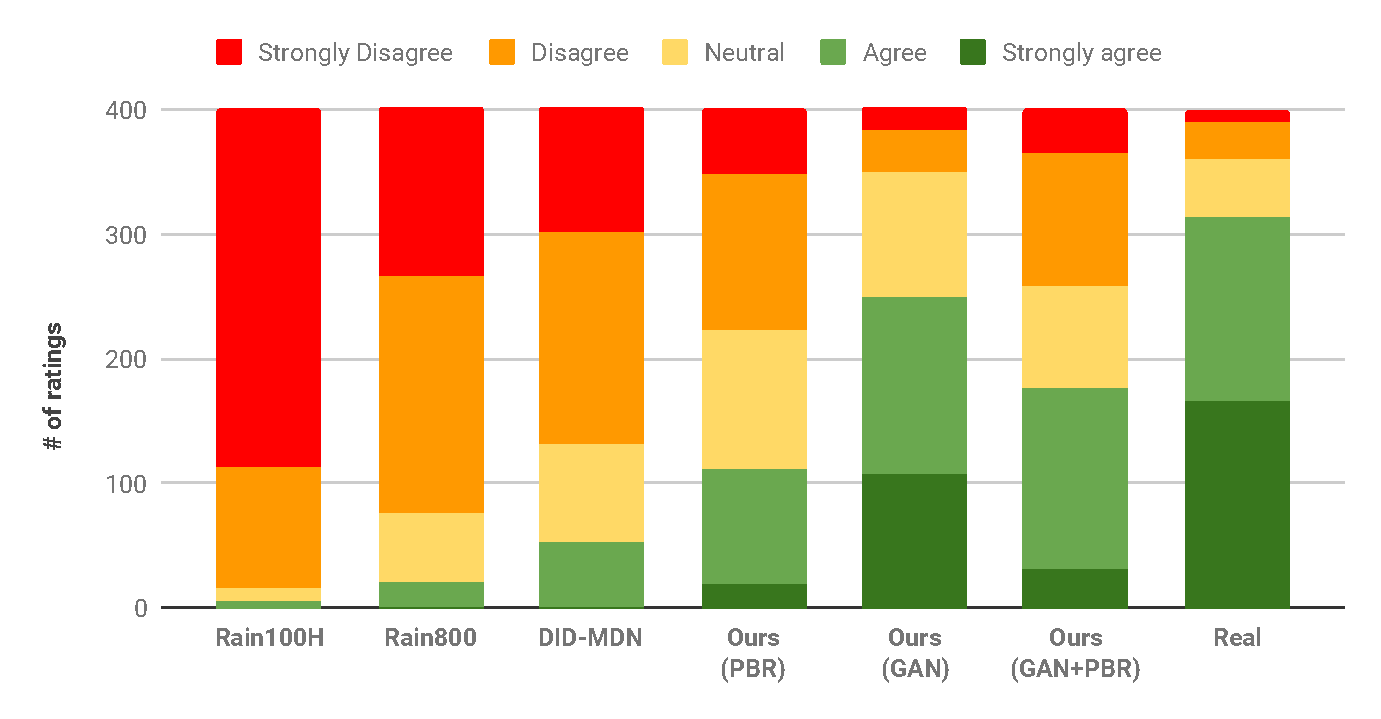
\includegraphics[width=\linewidth]{figures/user_study.pdf}
 \caption{\textbf{User study of rainy images realism.} The y-axis displays ratings to the statement "Rain in this image looks realistic". All of our approaches significantly outperform existing techniques.}
 \label{fig:user_study}
 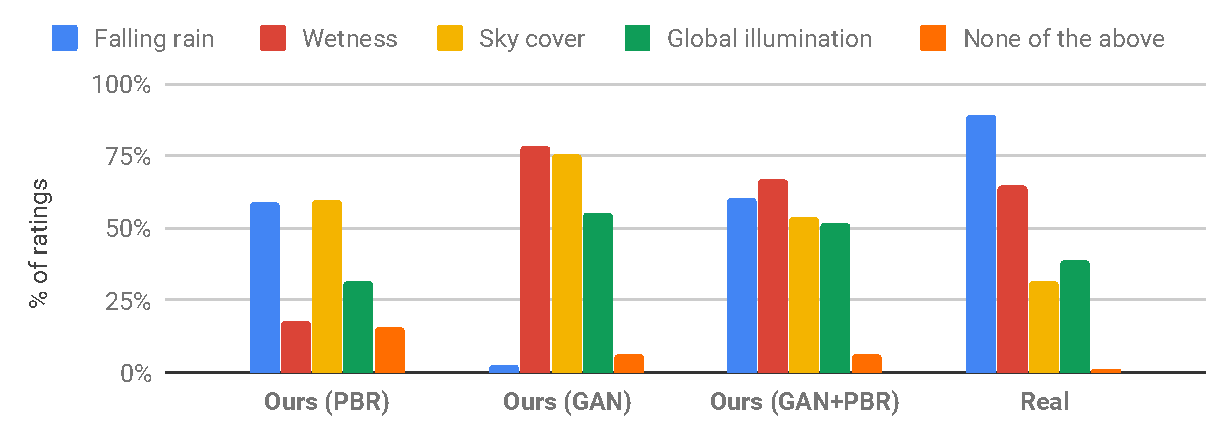
\includegraphics[width=\linewidth]{figures/user_study_followup.pdf}
 \caption{\textbf{User study on images characteristics conveying rain.} The y-axis displays ratings to the statement "Which of these qualities help in determining the realism of the rain".}
 \label{fig:user_study_followup}
\end{figure}

To evaluate the perceptual quality of our rain renderings, we conducted two user studies. In the first, users were shown one image at a time, and asked to rate if rain looks realistic on a 5-point Likert scale. A total of 42 images were shown, that is 6 for each of the following: real rainy photographs, ours (PBR, GAN, GAN+PBR), and previous approaches \cite{yang2017deep,zhang2018density,zhang2019image}. Answers were obtained for a total of 67 participants, aged from 22 to 75 (avg 37.0, std 14.2), with 32.8\% females.

From the Mean Opinion Score (MOS) in fig.~\ref{fig:user_study}, all our rain augmentation approaches are judged to be more realistic than any of the previous approaches. 
Specifically, when converting ratings to the [0,~1] interval, the mean rain realism is 0.77 for real photos, 0.44 for PBR, 0.68 for GAN, 0.52 for GAN+PBR, and 0.30/0.23/0.08 for~\cite{zhang2018density}/\cite{zhang2019image}/\cite{yang2017deep} respectively.
Despite physical and geometrical inconsistencies, the users consistently judged GAN images to be more realistic. This is in favor of using image-to-image translation rather than physics-based rendering for realism purposes.
However, for benchmarking or physical accuracy purposes, GAN+PBR allows us to have an arbitrary control on the rain amount at the cost of slightly lower realism.

In the second study, we asked respondents who participated in the first study to determine, for each of the same images as before (excluding images from the previous work), which visual characteristics influenced their decisions. 52 of the original participants responded, aged from 22 to 72 (avg 36.6, std 13.9) including 28.9\% females. 
Results are reported in fig.~\ref{fig:user_study_followup}.
We note that while \textit{falling rain} and \textit{wetness} are the main characteristics in real rain, GAN---judged the most realistic approach---fails to convey the \textit{falling rain} appearance but excels at rendering \textit{wetness}. The opposite is observed with PBR, though few users indicated \textit{wetness} (despite its absence). The GAN+PBR offers a trade-off balancing all characteristics. 
